\chapter{Implementation and Evaluation}

\section{Wrapping MonPoly}

\subsection{Performance}


\section{Policy Change}
% \tikzstyle{startstop} = [rectangle, rounded corners, 
minimum width=3cm, 
minimum height=1cm,
text centered, 
draw=black]
% fill=red!30]

\tikzstyle{io} = [trapezium, 
trapezium stretches=true, % A later addition
trapezium left angle=70, 
trapezium right angle=110, 
minimum width=3cm, 
minimum height=1cm, text centered, 
draw=black]
% , fill=blue!30]

\tikzstyle{process} = [rectangle, 
minimum width=3cm, 
minimum height=1cm, 
text centered, 
text width=3cm, 
draw=black] 
% fill=orange!30]

\tikzstyle{decision} = [diamond, 
minimum width=2cm, 
minimum height=1cm, 
text centered, 
text width=3cm,
draw=black]
% fill=green!30]
\tikzstyle{arrow} = [thick,->,>=stealth]

\begin{tikzpicture}[node distance=2cm]

% \node (start) [startstop] {Start};
% \node (in1) [io, below of=start] {Events get sent to wrapper};
\node (in1) [io] {Events get sent to wrapper};
\node (pro1) [process, below of=in1] {Wrapper checks JSON formatting};
\node (dec1) [decision, below of=pro1, yshift=-1.5cm] {JSON formatting correct?};

\node (pro2a) [process, below of=dec1, yshift=-2cm] {Convert JSON input to list of MonPoly style log strings for each time point};
\node (pro2b) [io, right of=dec1, xshift=3.2cm] {Abort and report issue to user};
\node (pro3) [process, below of=pro2a] {Send next time point to MonPoly};
\node (dec2) [decision, below of=pro3, yshift=-2cm] {Time point in order and predicates comply with signature?};
% \node (stop) [startstop, below of=pro3]{Stop};

% \draw [arrow] (start) -- (in1);
\draw [arrow] (in1) -- (pro1);
\draw [arrow] (pro1) -- (dec1);
\draw [arrow] (dec1) -- node[anchor=east] {yes} (pro2a);
\draw [arrow] (dec1) -- node[anchor=south] {no} (pro2b);
\draw [arrow] (pro2a) -- (pro3);
\draw [arrow] (pro3) -- (dec2);

\end{tikzpicture}

\begin{figure}
    \label{fig:flowchart}
    \centering
    % 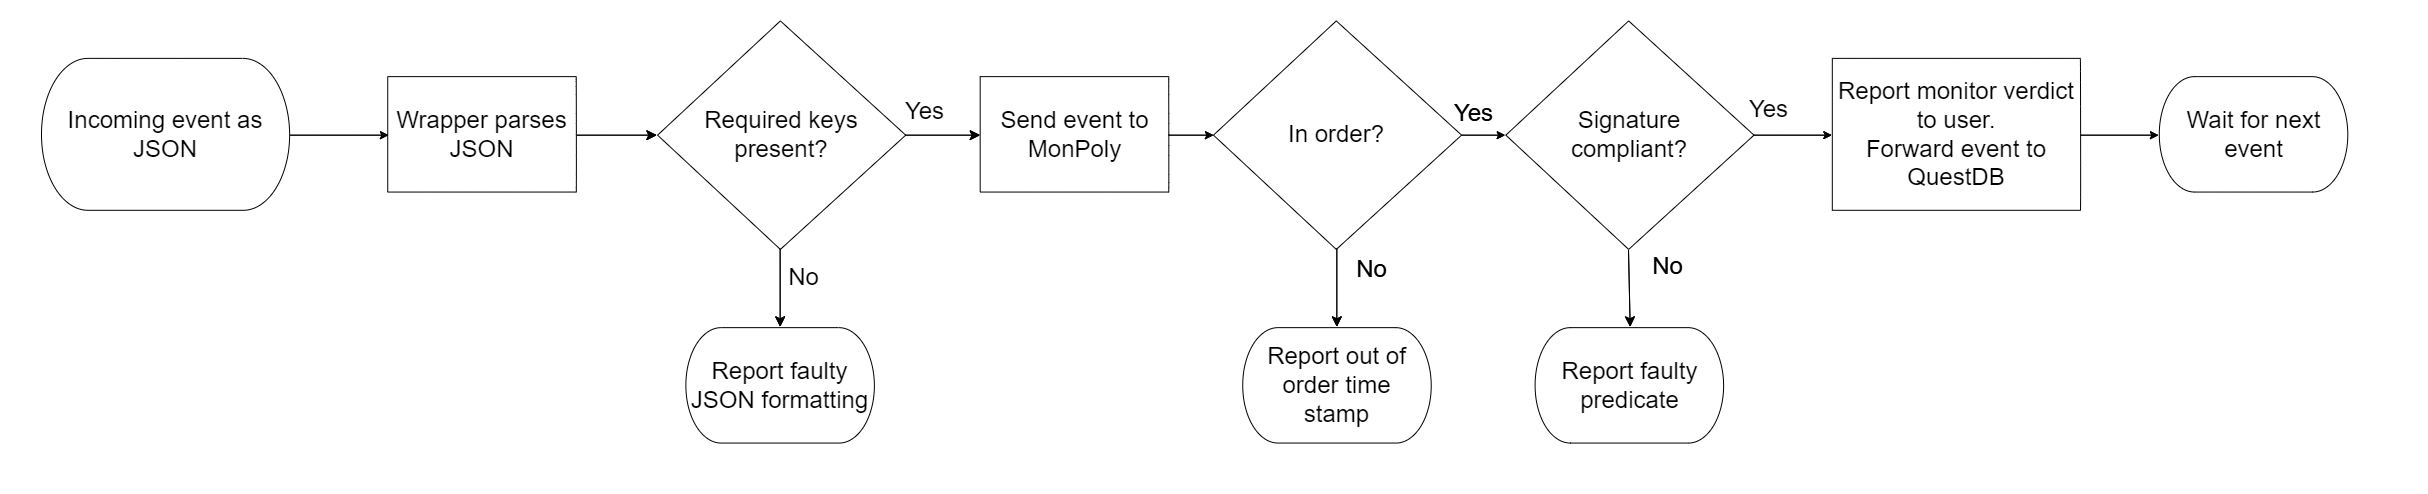
\includegraphics[width=110mm]{diagrams/flowchart.png}
    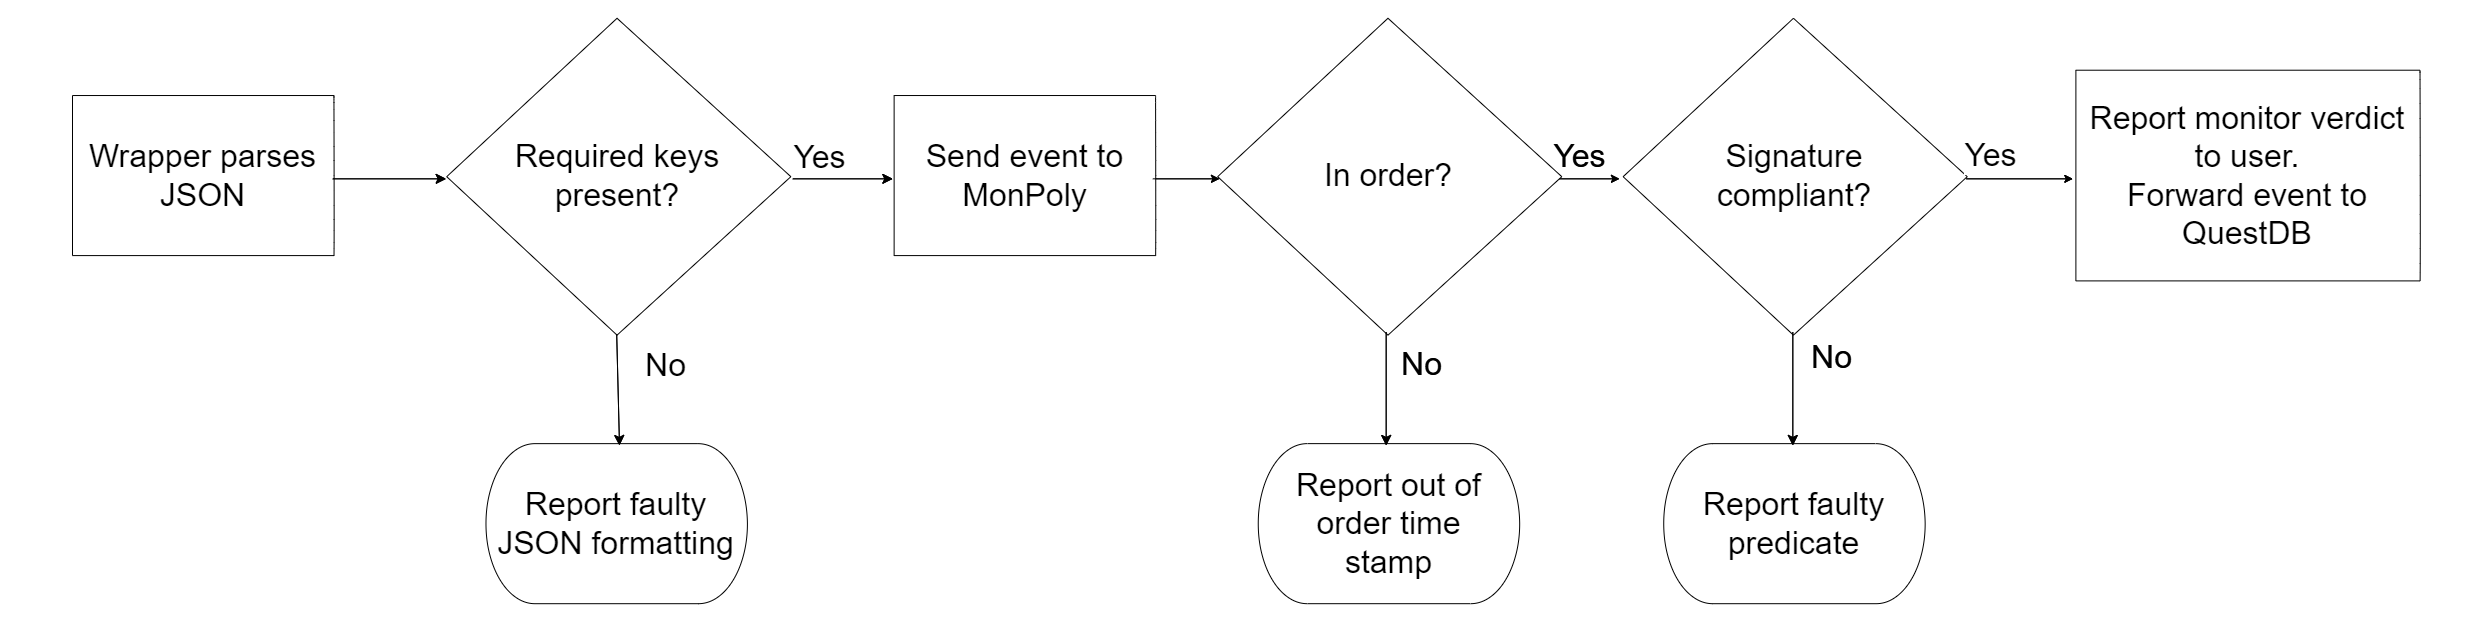
\includegraphics[width=\linewidth]{diagrams/flowchart-2.png}
    \caption{Control flow for a new event}
\end{figure}

This first version of a policy change functions by stopping the current monitor and starting a new one.
When starting the new monitor we want to restore the state of the old one.
We do this by querying old events from our database.
But we do not simply query for the entirety of the database.
We make two optimizations.
First we use relative intervals and second we make use of constant values.
For each predicate occurring in a formula we look for constant attributes in its occurrences.
For every predicate and its potential occurrences with different constant values we then compute an over approximation of the relative interval.
We use this information to create a SQL query that only queries the constant values combined with the interval.
This way we minimize the amount of data that the new monitor has to read and process.


\section{Partial Policy Updates}